\documentclass[a4paper 12pts]{article}
\usepackage[utf8]{inputenc}
\usepackage[T1]{fontenc}
\usepackage[francais]{babel}
\usepackage{graphicx}


\title{Documentation Technique : iRover}

\author{}

\begin{document}

\maketitle


\begin{figure}[h]
   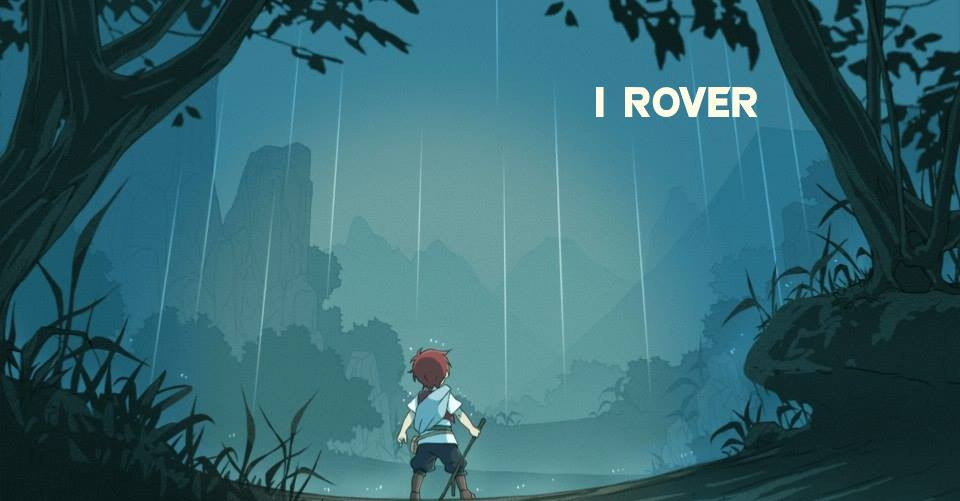
\includegraphics[width=350pt]{Illustration/proj_irover.jpg}
	\caption{iRover, l'histoire d'un héros qu'on appellait robot}
\end{figure}



\newpage


\renewcommand{\contentsname}{Sommaire} 
\tableofcontents

\newpage








\section{Manuel Documentation Technique}


\vspace{2cm}

Cette partie est dédiée aux développeur
%expliqué à quoi sert cette documentation


\subsection{Les personnages}


\subsubsection{Le robot, Rover}

\subsubsection{les ennemis}



\subsection{les coffres}


\subsection{les clé}


\subsection{L'environnement}


\subsection{La gestion des évênements}


\subsubsection {Rencontre avec un ennemi} 


\subsubsection {Ouvertude d'un coffre}


\subsubsection {Ramasser une clé}

 
\subsection{l'interface utilisateur}

\subsection{IA}

\subsubsection{path finding}

\subsubsection{découverte de la carte}

\subsection{condition fin de jeu}





\end{document}

